\mysubsubsection{Optical Flow}


% \hang{figure file missing}
\begin{figure}[tb]
  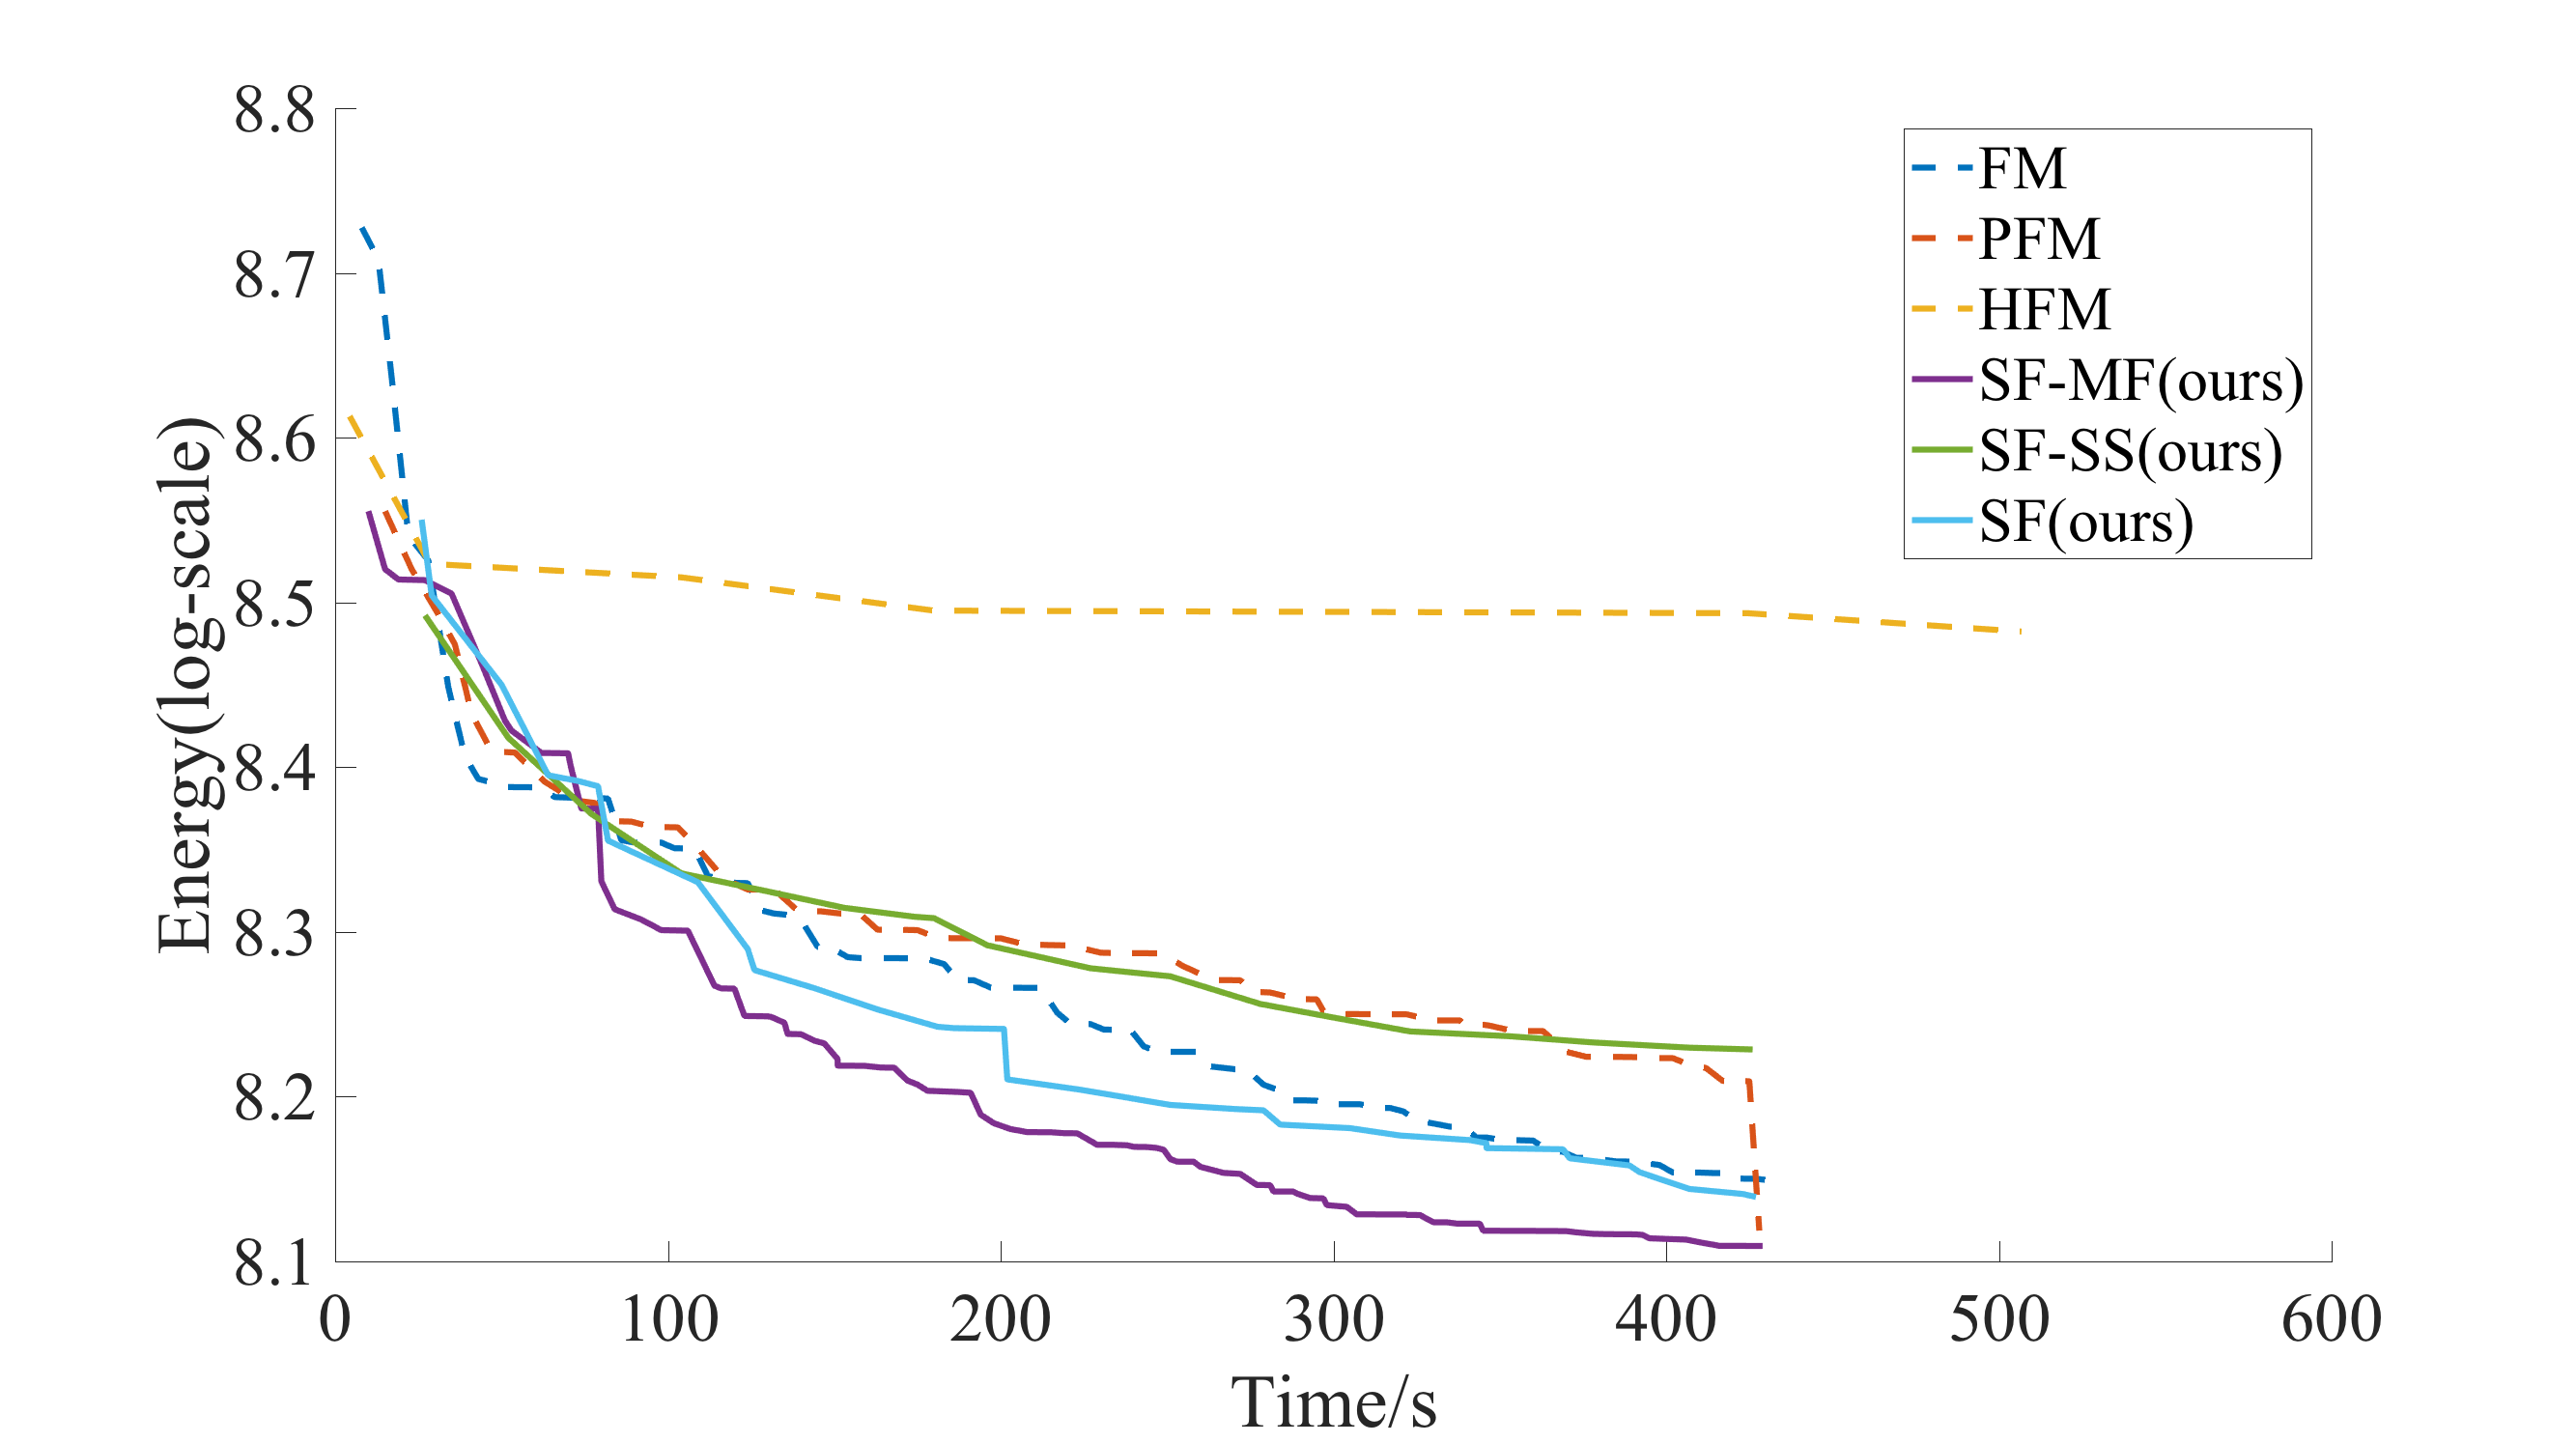
\includegraphics[width=\columnwidth]{figure/optical_flow_convergence.png}
  \caption{The energy minimization process for optical flow estimation of different methods. FS-MF has the best performance because of the solution sharing in early stage.}\label{fig:optical_flow_convergence}
\end{figure}
\begin{figure}[tb]
  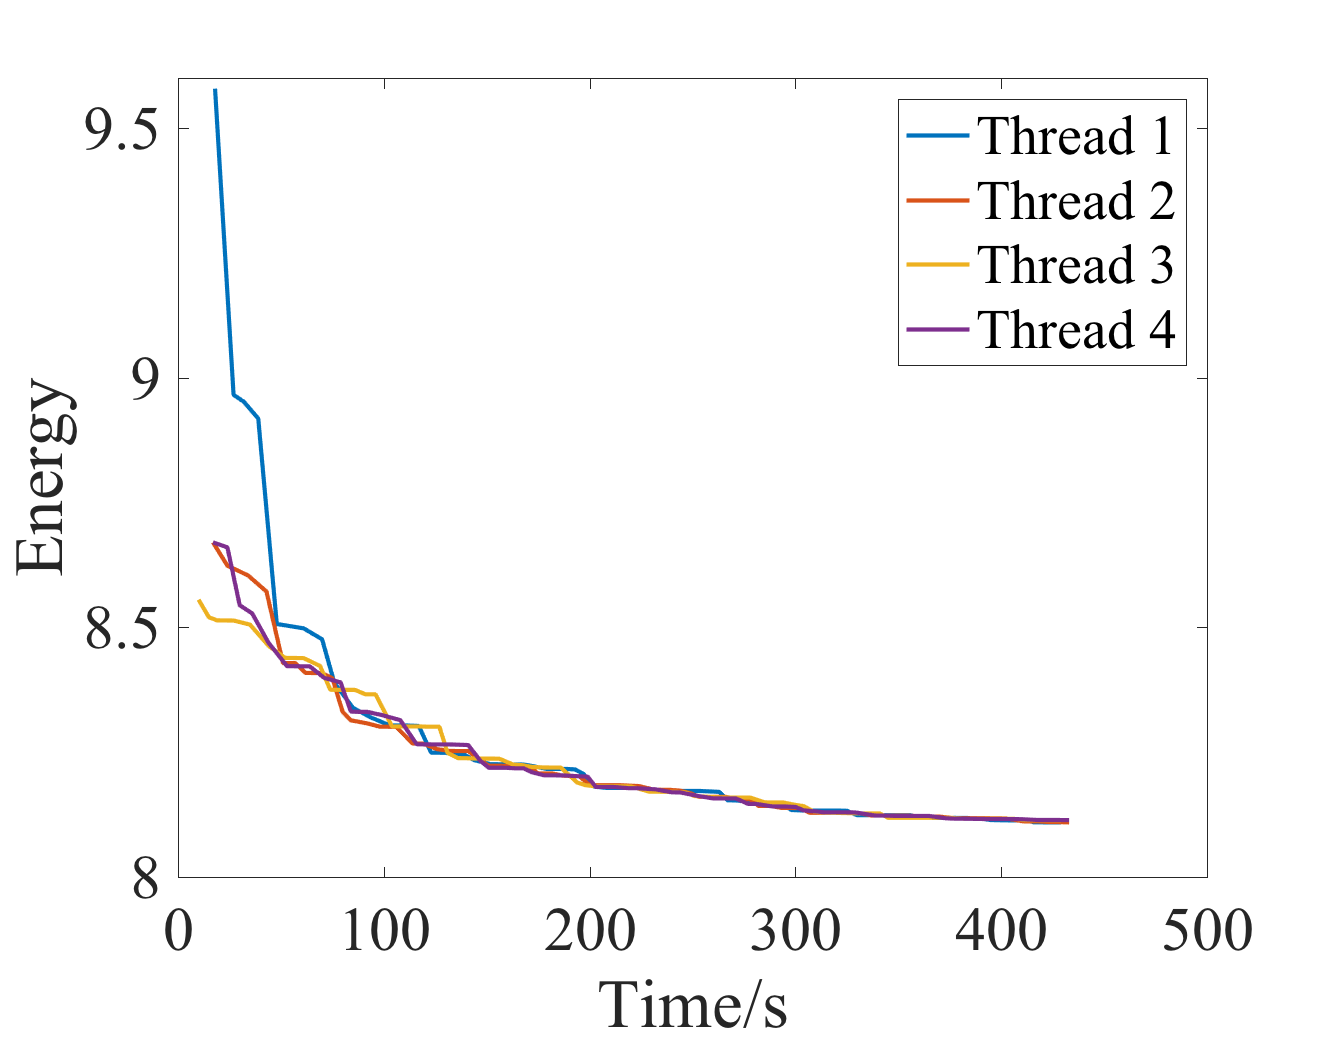
\includegraphics[width=0.5\columnwidth]{figure/optical_flow_SF_MF_threads.png}
  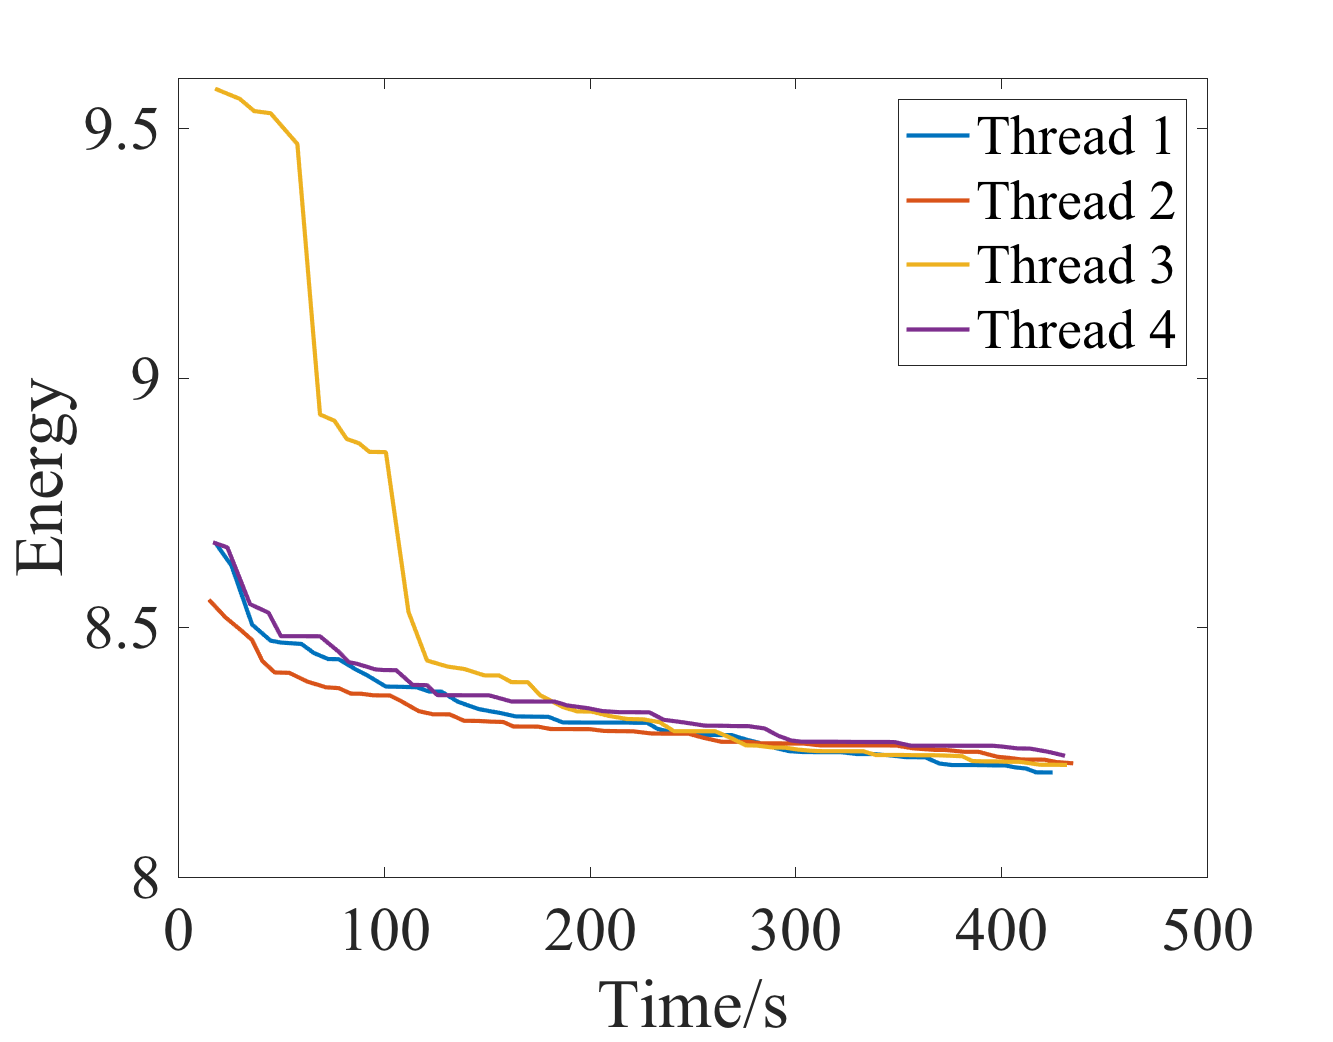
\includegraphics[width=0.5\columnwidth]{figure/optical_flow_PFM_threads.png}
  \caption{Per thread energy. The left and right figures show the energy minimization process on each working thread of our method in SF-MF configuration and parallel fusion move, respectively.}\label{fig:optical_flow_by_threads}
\end{figure}
\begin{figure}[tb]
  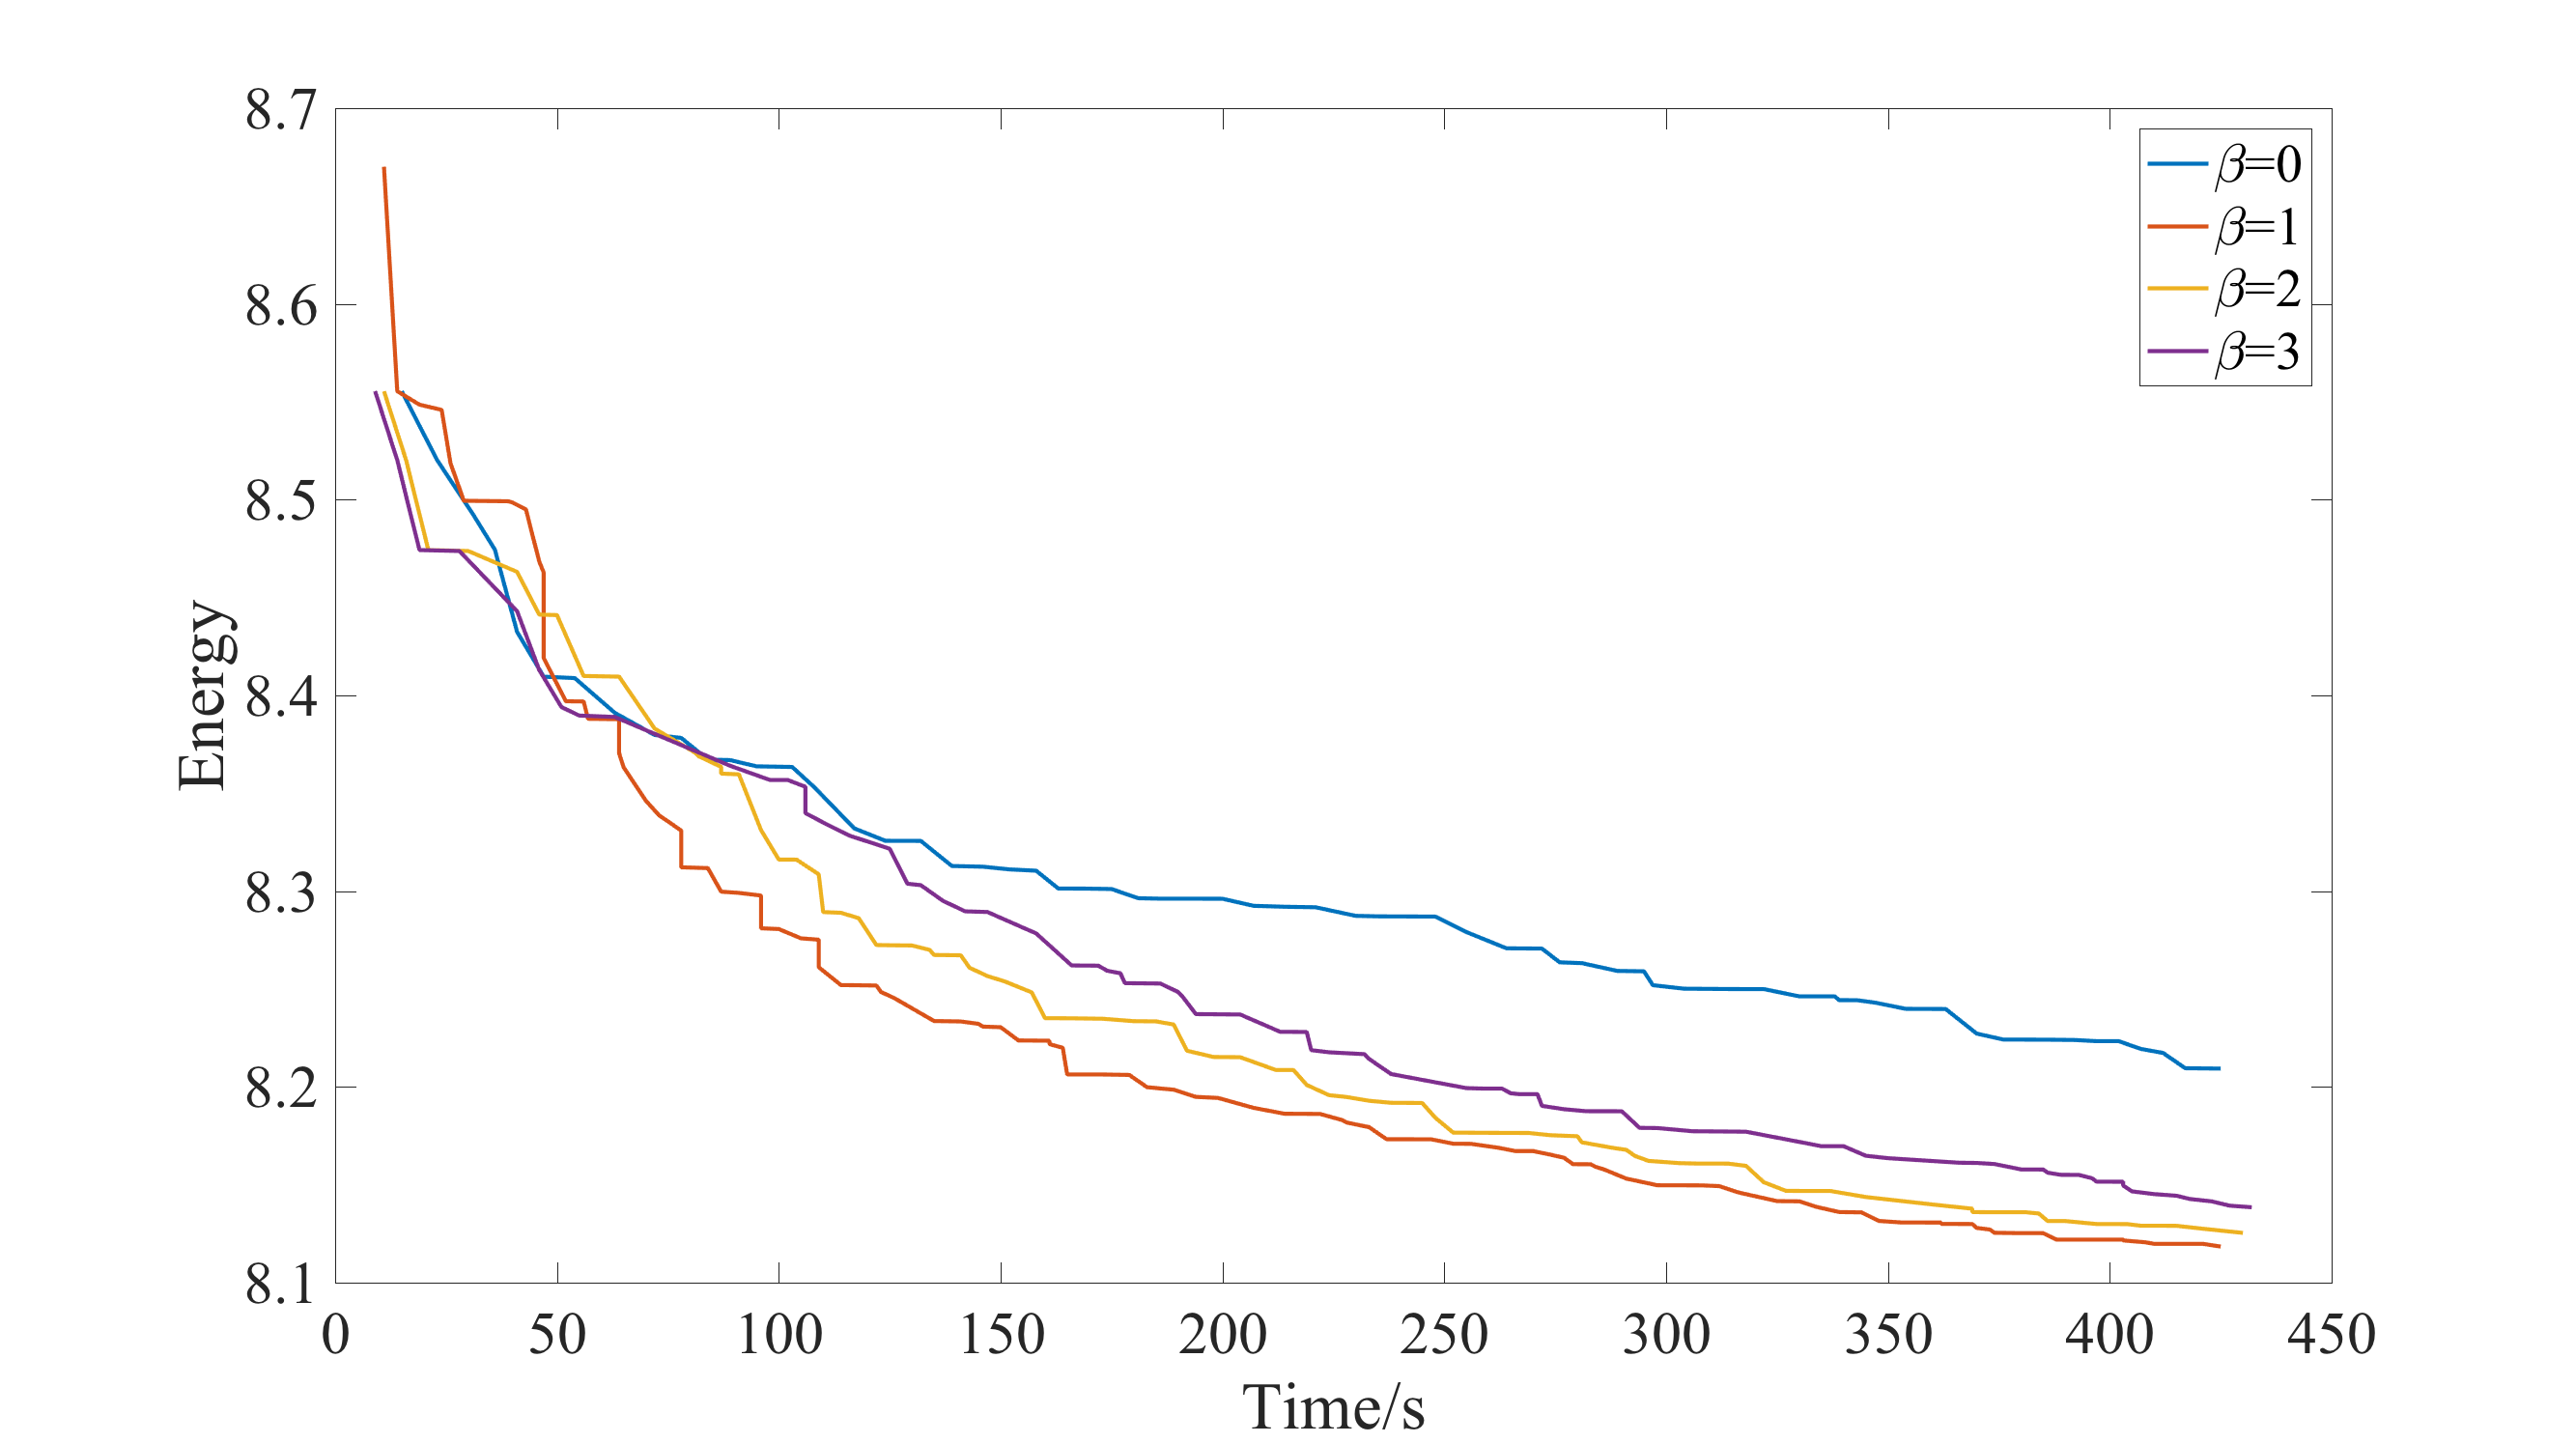
\includegraphics[width=\columnwidth]{figure/optical_flow_by_beta.png}
  \caption{The energy minimization process for optical flow estimation with different $\beta$ values. Solution sharing generally makes energy minimization faster, but more solution sharing also means less time for exploring new solution proposals.}\label{fig:optical_flow_by_beta}
\end{figure}
\begin{figure}[tb]
  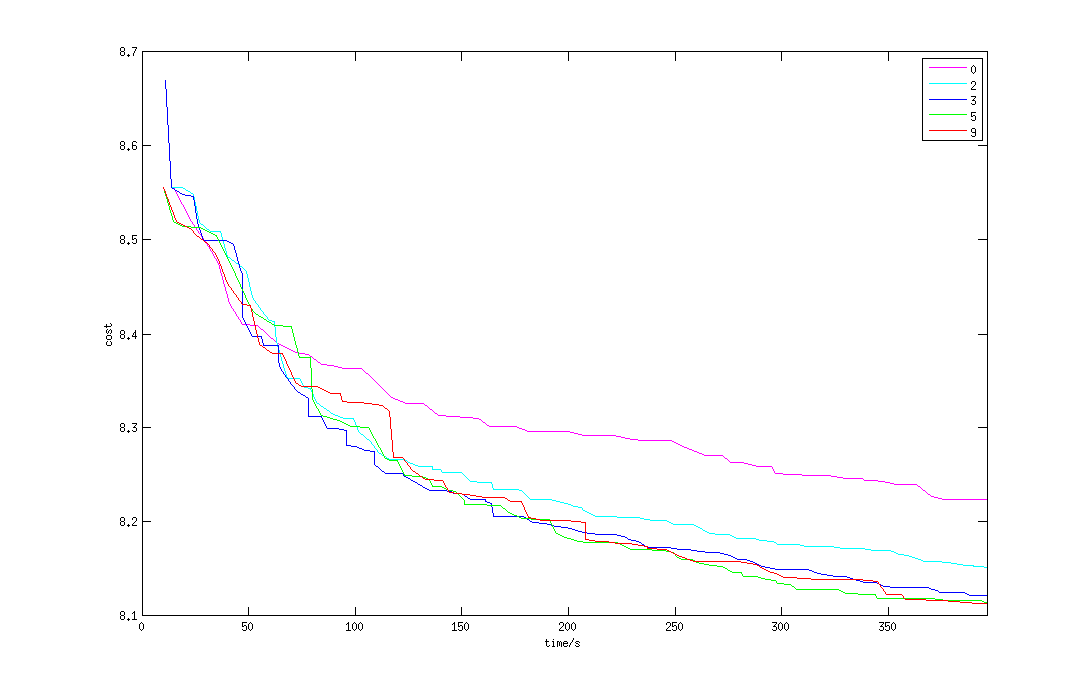
\includegraphics[width=\columnwidth]{figure/optical_flow_by_interval.png}
  \caption{The energy minimization process for optical flow estimation with different solution sharing frequency. Solution sharing generally makes energy minimization faster, but frequent solution sharing also means less time for exploring new solution proposals.}\label{fig:optical_flow_by_beta}\label{fig:optical_flow_by_interval}
\end{figure}

Figure \ref{fig:optical_flow_convergence} illustrates the convergence rate of three competing methods (alpha expansion, parallel alpha expansion, hierarchical fusion) against
our swarm fusion method. From the figure we can observe that, both conducting binary fusion, FS-MF finds lower energy faster than PFM. This is because some solution proposals are more effective than others, so once a thread grabs an effective solution proposal, it find a lower energy quickly. Since there is no solution sharing in PFM model, other threads cannot share this lower energy state, and keeps working on its own state. On the other hand, FS-MF allows solution sharing, so once a thread grabs an effective solution proposal and moves to a lower energy state, other threads can share this lower energy state. To further demonstrate what is happening here, we plot per thread energy in PFM and FS-MF in figure \ref{fig:optical_flow_by_threads}. As we can see from the plots, in PFM model, one thread finds lower energy state faster than others, while other threads keep working at their own energy state. But in FS-MF model, all threads exchange information about the lowest energy state and work on improving the lowest energy state together. So there are more chance of finding effective proposals faster. Since the solution for optical flow can be locally improved by each thread, the final merging of PFM can effectively fuse good local results in different threads together and achieve a similar energy state with FS-MF model. But since FS-MF model shares information in the middle, a final merging becomes less necessary. Same comparison holds for FS-SS and FS. The multi-way fusion is ineffective in this problem setting since solution proposals are relatively independant and fusing multiple solutions together using TRW-S~\cite{TRW-S} is less efficient than fusing them one by one using~\cite{QPBO}.

They are two factors influencing solution sharing: 1) \textit{the number of solutions to share} and 2) \textit{the solution sharing frequency}. Both factors are controlled by $\beta$. As mentioned in the section \label{optical_flow}, we use $\beta = 1$ once in every five iterations and use $\beta = 0$ for all other iterations. This means we share one solution in every five iterations. To further understand the effect of solution sharing, we did two other experiments for comparison. In one experiment, we use $\beta = {0, 1, 2, 3}$ in every five iterations and $\beta = 0$ for other iterations (when $\beta = 0$, it is same with PFM without final merging). While keeping all other factor same, we plot the energy minimization process in figure \ref{fig:optical_flow_by_beta}. As shown in the figure, energy generally decreases faster with solution sharing. But since we need to perform one fusion for sharing each solution, sharing more solution decreases efficiency in this problem setting. While sharing multiple solutions might be useful in some other problem setting as it means each thread can get more global information early. In another experiment, we change the number of iterations between two consecutive solution sharing iterations (the number of zero $\beta$ between two non-zero $\beta$) and plot the energy minimization process in figure \ref{fig:optical_flow_by_interval}. From this figure, we can see that although solution sharing generally speeds up the optimization process, sharing solution too frequently is not a good practice. This is because when we share solution frequently, we have less time for generating and fusing new proposals. A good choice of the solution sharing frequency depends on specific problem setting.
